\documentclass{article}


% if you need to pass options to natbib, use, e.g.:
% \PassOptionsToPackage{numbers, compress}{natbib}
% before loading nips_2018

% ready for submission
\usepackage{nips_2018}

% to compile a preprint version, e.g., for submission to arXiv, add
% add the [preprint] option:
%\usepackage[preprint]{nips_2018}

% to compile a camera-ready version, add the [final] option, e.g.:
%\usepackage[final]{nips_2018}

% to avoid loading the natbib package, add option nonatbib:
% \usepackage[nonatbib]{nips_2018}

\usepackage[utf8]{inputenc} % allow utf-8 input
\usepackage[T1]{fontenc}    % use 8-bit T1 fonts
\usepackage{hyperref}       % hyperlinks
\usepackage{url}            % simple URL typesetting
\usepackage{booktabs}       % professional-quality tables
\usepackage{amsfonts}       % blackboard math symbols
\usepackage{nicefrac}       % compact symbols for 1/2, etc.
\usepackage{microtype}      % microtypography
\usepackage{textcomp}
\usepackage{amsmath}
\usepackage{graphicx}
\usepackage{multirow}
\usepackage{multicol,color}

\title{Experimental Secure Multi-Party Computation on Real Data using SPDZ}

% The \author macro works with any number of authors. There are two
% commands used to separate the names and addresses of multiple
% authors: \And and \AND.
%
% Using \And between authors leaves it to LaTeX to determine where to
% break the lines. Using \AND forces a line break at that point. So,
% if LaTeX puts 3 of 4 authors names on the first line, and the last
% on the second line, try using \AND instead of \And before the third
% author name.

\author{
  Valerie Chen\\
  Yale University\\
  %% Address?? \\
  \texttt{v.chen@yale.edu} \\
  \And
  Valerio Pastro\\
  Yale University\\
  \textt{valerio.pastro@yale.edu}\\
  %% examples of more authors
  \And
  Mariana Raykova \\
  Yale University \\
  %% Address?? \\
  \texttt{mariana.raykova@yale.edu} \\
  %% \AND
  %% Coauthor \\
  %% Affiliation \\
  %% Address \\
  %% \texttt{email} \\
  %% \And
  %% Coauthor \\
  %% Affiliation \\
  %% Address \\
  %% \texttt{email} \\
  %% \And
  %% Coauthor \\
  %% Affiliation \\
  %% Address \\
  %% \texttt{email} \\
}

\begin{document}

\maketitle

\begin{abstract}
  Secure Multi-Party Computation (MPC) is an area of theoretical cryptography research that has the power to revolutionize computation between shared parties holding private data. However theoretical protocols are often not scalable and efficient given large quantities of real world data. This project investigates an MPC protocol called SPDZ which is secure against malicious adversaries in comparison to two other semi-honest MPC protocols Obliv-C and SecureML in machine learning and regression applications. We demonstrate its potential to be used in real world applications with experiments to show that it outperforms the other two methods while maintaining a more rigorous level of security.
\end{abstract}

\section{Introduction}

Regression analysis and other machine learning techniques aim to build a model that fits a set of predictors to the dependent variable. Models built from a large set of collected data can be used to predict future behavior. With the advent of big data, it is becoming increasingly common for entities to store vast amounts of user data, run regression analyses and build models of this data to gain insights. A desired use case could be, for example, the Center for Disease Control is interested in identifying disease outbreak and many individual hospitals have their own patient data which could benefit this study. The problem is that openly sharing this data for prediction or model-building purposes would be against modern day privacy laws as it would leak private individual data [2]. This application of secure MPC is one that would be extremely valuable in today\textquotesingle s world.

\subsection{Multi-Party Computation}

Secure MPC addresses this problem by providing a mechanism through which different parties supply their data for joint computation without revealing individual values from each database or even intermediate values. This need for MPC motivates our study to bridge theory and application through experiments on real-world data. 

In general, MPC protocols predominantly come in two forms: security against semi-honest and malicious adversaries [4]. In semi-honest security, a more naive model, it is assumed that the party will follow the protocol as specified but will merely gather information intermediate values. Typically semi-honest security is more efficient on computation as it has fewer requirements. In malicious security, dishonest parties may attempt to deviate from the specified protocol, and the protocol must be able to detect such cheating and abort the computation - thus any successful output is guaranteed to have privacy preserved. This notion can be rigorously proved. 

For this study, we chose the SPDZ framework [1,5], which ensures against malicious security, and compare against two semi-honest methods Obliv-C [7] and SecureML [6]. SPDZ performs the checks necessary to detect dishonest parties through using random data in the hopes of making computation more efficient. Obliv-C is based on Yao\textquotesingle s garbled circuits and [3] introduces optimizations on inner products and algorithmic modifications to speed up regression calculation. SecureML\textquotesingle s focus is with developing MPC-friendly alternatives to non-linear activation functions which are often intensive to compute as well as vectorization techniques in a shared setting. 

Since secure computation slower and could be limited in accuracy when compared to computation in plaintext, there are a number of modifications to plaintext algorithms that can be made to obtain a reasonable degree of accuracy in more efficient time.

\section{ML Functionalities}

Our goal was to conduct a thorough investigation of the SPDZ framework in the applications of regression and machine learning algorithms in a similar fashion to that done in  [3,6], evaluating in terms of runtime and accuracy. The main algorithms that we considered were, LDLT Decomposition, Cholesky, Conjugate Gradient Descent (CGD), Stochastic Gradient Descent (SGD), Logistic Regression. The algorithms were implemented in the SPDZ framework as a proof-of-concept as well as in python as a plaintext verification of the accuracy of the secure version.

\subsection{Direct vs. Iterative Decomposition}

LDLT and Cholesky are both variants of direct decomposition methods which decompose a Hermitian, positive-definite matrix into a lower triangular matrix and its conjugate transpose. The algorithms are cubic in complexity with asymptotic run time of $O(d^3)$. This can become inefficient to work with when looking at real world data that has large number of features and entries. The difference between LDLT and Cholesky is that Cholesky requires a square root. In MPC, non-linear functions like square roots are difficult to represent. Thus we looked at an iterative Newton method as a way of approximating the square root in SPDZ to solve for $x_i$ where $x_{i}^2 = S$:

\[
x_{n+1} = \frac{1}{2} (x_{n} + \frac{S}{x_{n}})
\]

In terms of an iterative approach to regression, [3] proposed a modification for the normalization in the iterative version of CGD that would be more stable with fixed-point numbers. We applied the same algorithm to SPDZ to see if the same modification would work. The goal of comparing iterative versus a direct method would be to justify the potential accuracy trade off for a much smaller run time.

\subsection{Gradient Descent}

Stochastic gradient descent is also an iterative method that minimizes a differentiable cost function and is the driving mechanism behind most neural networks. In linear regression the cost function is derived from the mean squared error. The update consists of forward propagation to calculate the predicted output $y_i^* = x_i \cdot w$ and a backward propagation phase to adjust weights accordingly given differential error and learning rate $\alpha(y_i^*-y_i)x_{ij}$ for an update function of $w_j = w_j  - \alpha(x_i \cdot w *-y_i)x_{ij}$.

We implemented mini-batch SGD so the weights would converge more quickly and in smoother fashion to the minimum. Since SPDZ had limited functionality for matrix manipulations and vectorization, we were not able to take advantage of the time speed-ups in this sense. The update function for the batched version is: 
\[
 w = w - \frac{1}{|B|} \alpha X^{T}_{B} \times (X_{B} \times w - Y_{B})
\]

\subsubsection{Non-Linear Activations}

Logistic regression models a binary dependent variable. For logistic regression, the activation function is defined as the logistic function $f(u) = \frac{1}{1+e^-u}$. Using the cross entropy function, we derive a similar update function for mini-batched SGD as $ w = w - \frac{1}{|B|} \alpha X^{T}_{B} \times f(X_{B} \times w - Y_{B})$. To approximate the activation function, [2] proposed this following piecewise function:

\[
  f(u) =
  \begin{cases}
                                   0 & \text{if $u < -0.5$} \\
                                   u + 0.5 & \text{if $-0.5 \leq u \leq 0.5$} \\
1 & \text{if $u > 0.5$}
  \end{cases}
\]

We compare the results of this MPC-friendly piecewise function to a more standard approximation approach of taking the Taylor Series expansion to varying degrees.

\section{Experiments}

\subsection{Experimental Setup}

The main metrics of evaluations were the error in accuracy and the RMSE for prediction error. We varied the precision after the decimal point (32 and 64 bits) or less depending on the comparison.

To simulate the players, we needed to identify a source of data. We used both a combination of existing, well-known datasets (MNIST, Arcene, and 9 other UCI open-source datasets) as well as synthetically generated data. The advantage to using synthetic data is being able to control characteristics of the data like the dimensions (d = 10, 20, 50, 100, 200, 500), condition number (cd = [1,10]), and number of examples (n = 1000, 100000).

Typically in a two player setting, both parties were run on one machine but we also performed tests where both parties were deployed on separate Amazon EC2 m4.large instances. It is important to note that the distribution of players across machine only affects runtime and not the accuracy of the results. We also looked at up to four parties as a form of validation of the SPDZ protocol.

\subsection{Results}

This section presents empirical results for real-world and synthetic data evaluated on the SPDZ protocol, comparing the five different algorithms in terms of accuracy and run time for various parameters. 

For LDLT, Cholesky and various iterations of CGD, we evaluated on synthetically generated data of varying sizes and condition numbers, since the data needed to be of a specific form. The direct decomposition methods grew exponentially in run time on the log scale as the matrix size increased, which means that it is not suitable for large size real data. Alternatively, the iterative CGD runtime increases at a much slower rate. In the middle column of Figure 2, we find that about 20 iterations is sufficient to reach maximum accuracy given the number of allocated bits even with varying condition numbers, meaning the data might not be as well-formed. Particularly for the 64-bit case, shown on the bottom right, the accuracy is identical for CGD after 15 iterations and Cholesky/LDLT.

\begin{figure}[h!]
\centering
  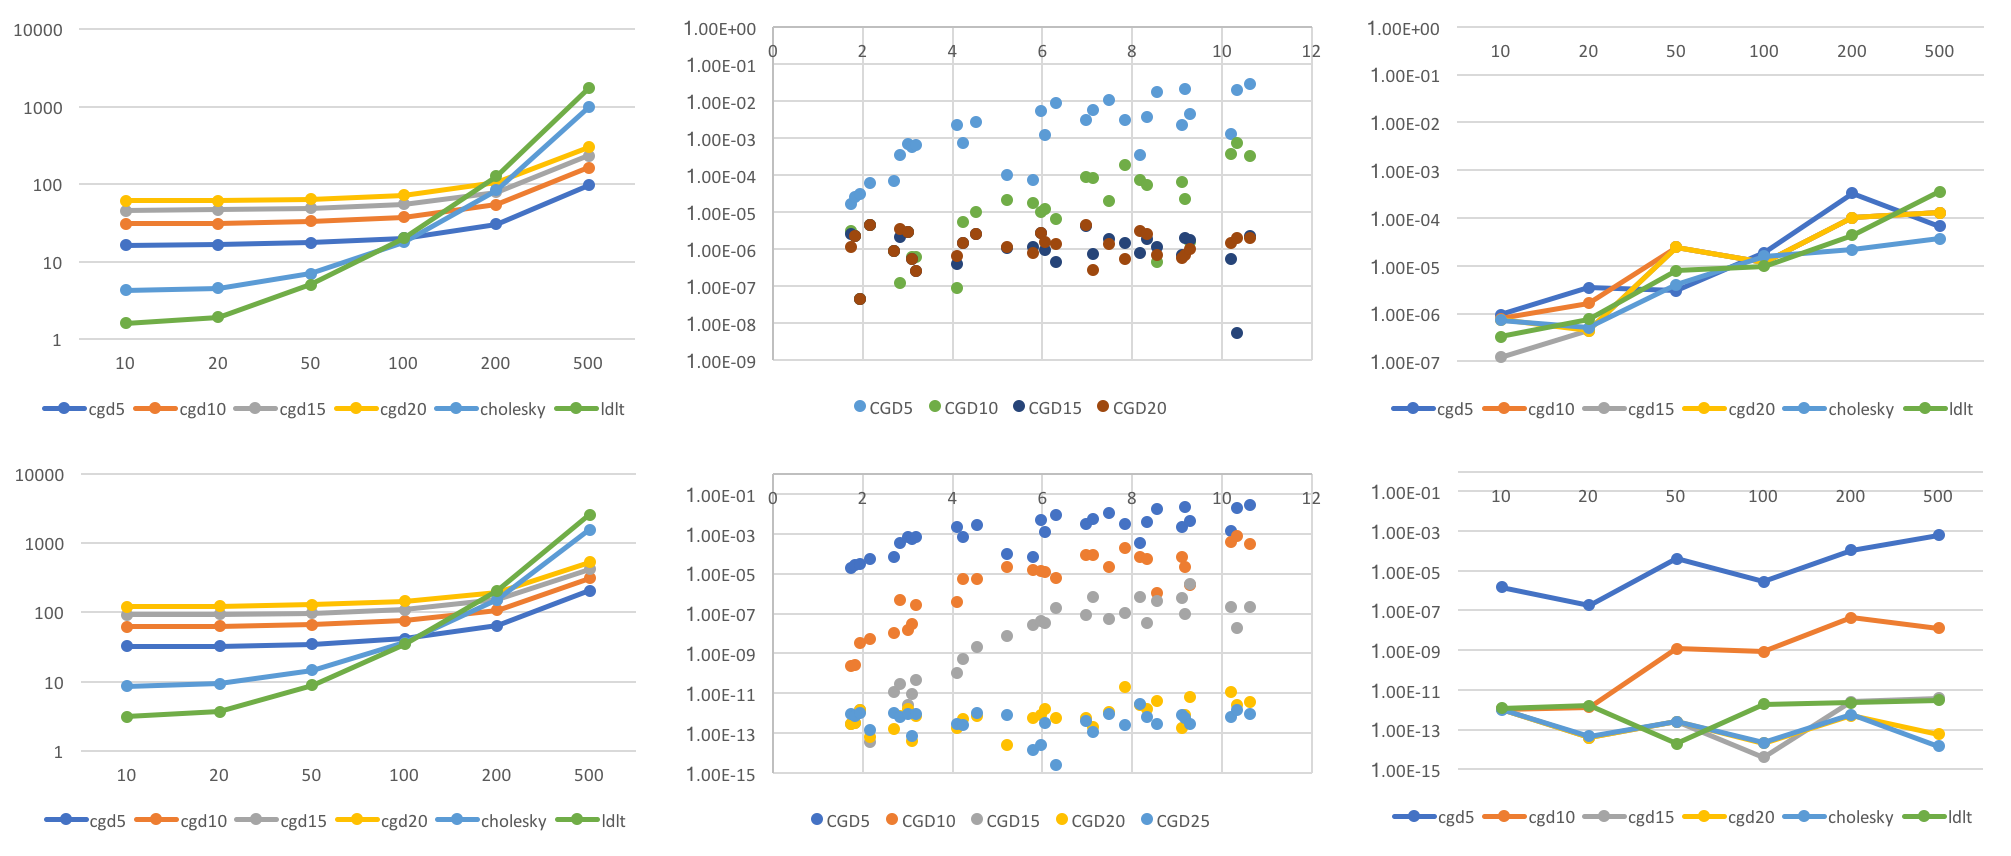
\includegraphics[scale=0.4]{allregression.png}
  \label{fig:result4}
    \caption{(Left) Run time comparison in seconds as a function of input dimension. (Middle) Condition number as a function of accuracy. (Right) Accuracy as a function of the input dimensionality $d$. (Top) Fixed-point numbers with the $b = 80$ bits, with 60 in the fractional part. (Bottom) $b = 41$, with 28 in the fractional part}
\end{figure}

Figure 2, which compares MNIST and Arcene results, demonstrates that the number of bits of precision needed to get good accuracy is highly dependent on the dataset. For MNIST, 13 bits was sufficient to match plaintext accuracy but 28 bits were needed for Arcene. The MNIST data contains only 784 features while there are 10,000 in the Arcene data, thus the larger the feature set the more bits needed. While the numbers in the MNIST data ranged from 0 to 9, [6] only used the 0s and 1s labels from the dataset, thus reducing it to a binary problem. We also compared the root mean squared error (RMSE) of SGD on 9 UCI open-sourced datasets of ranging sizes to results in [3] and found lower RMSE results. Due to limited space, these results are not presented.


\begin{figure}[h!]
\centering
  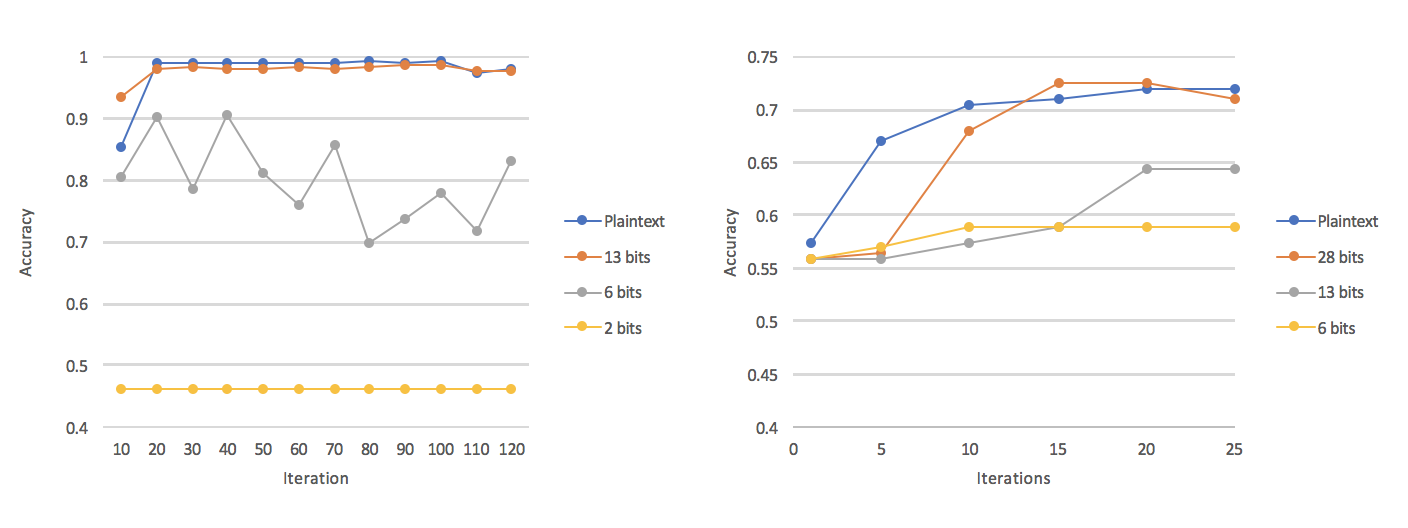
\includegraphics[scale=0.6]{mnistarcene.png}
  \label{fig:result4}
   \caption{Varying number of bits and recreating results for MNIST (left) and Arcene (right) in [2].}
\end{figure}

In terms of logistic regression, for SPDZ, we did not find that the new activation function was a better alternative to taking a Taylor Series approximation for the exponential function as shown in Table 1. We found that for SPDZ, which is based on arithmetic circuits, the extra time to take a few extra degrees in the approximation was negligible.  

\begin{table}[h!]
\caption{Comparing the validation accuracy for different activation functions for logistic regression for a fixed train/test dataset using 32 bits (for 1 epoch and learning rate of 0.01)}
\centering
\label{my-label}
\begin{tabular}{@{}lllllll@{}}
\toprule
       & Plaintext & New Activation function & \multicolumn{4}{l}{Polynomial Approximation} \\
       &           &                         & degree 2  & degree 5  & degree 7 & degree 10 \\ \midrule
MNIST  & 99.9\%    & 95\%                    & 97\%      & 85\%      & 91\%     & 99.5\%    \\
Arcene & 72.0\%    &           44.0\%              &   44.0\%        &    44.5\%       &    65\%      &    72\%       \\ \bottomrule
\end{tabular}
\end{table}

\subsection{Comparison}

\begin{table}[h!]
\caption{Runtime results against }
\centering
\begin{tabular}{@{}llcl@{}}
\toprule
\multicolumn{1}{c}{Datasets}                                           & \multicolumn{3}{c}{Runtime (seconds)}                                      \\ \midrule
CGD (64 bit)                                                           & \multicolumn{1}{c}{Ours} & Ours (EC2) & \multicolumn{1}{c}{Obliv-C}        \\ \midrule
d=100                                                                  & 144                      & 243        & \textgreater $10^4$ \\ \midrule
d=500                                                                  & 527                      & 2701       & \textgreater $10^3$ \\ \midrule
\multirow{2}{*}{\begin{tabular}[c]{@{}l@{}}SGD: \\ MNIST\end{tabular}} & \multicolumn{1}{c}{Ours} & \multicolumn{2}{c}{SecureML}                    \\ \cmidrule(l){2-4} 
                                                                       & 10200                    & \multicolumn{2}{c}{10330}                       \\ \bottomrule
\end{tabular}
\end{table}

Through this work, we demonstrated that SPDZ outperforms other protocols Obliv-C and SecureML in terms of accuracy, as evidenced in Table 2, efficiency, and security. In future work, we plan to expand the selected algorithms beyond linear and logistic regression to include neural networks and deep neural networks. This investigation into the applicability of secure MPC on real world data demonstrates its potential change the way data is used in a variety of applications in today\textquotesingle s world.

\section*{References}

\small

[1] Damg\aa rd, I., Keller, M., Larraia, E., Pastro, V., Scholl, P., \& Smart, N. P. (2013). Practical covertly secure MPC for dishonest majority?or: breaking the SPDZ limits. {\it European Symposium on Research in Computer Security}, pp.\ 1-18.

[2] Du, W., \& Atallah, M. J. (2001). Secure multi-party computation problems and their applications: a review and open problems. {\it Proceedings of the 2001 workshop on New security paradigms}, pp.\ 13-22. ACM.

[3] Gasc\'{o}n, A., Schoppmann, P., Balle, B., Raykova, M., Doerner, J., Zahur, S., \& Evans, D. (2017). Privacy-preserving distributed linear regression on high-dimensional data. {\it Proceedings on Privacy Enhancing Technologies, 2017(4)}, pp.\ 345-364.

[4] Hazay, C., \& Lindell, Y. (2010). A Note on the Relation between the Definitions of Security for Semi-Honest and Malicious Adversaries. {\it IACR Cryptology ePrint Archive}, pp.\ 551.

[5] Keller, M., Scholl, P., \& Smart, N. P. (2013). An architecture for practical actively secure MPC with dishonest majority. {\it Proceedings of the 2013 ACM SIGSAC conference on Computer \& communications security}, pp.\ 549-560. ACM.

[6] Mohassel, P., \& Zhang, Y. (2017). SecureML: A system for scalable privacy-preserving machine learning. {\it 38th IEEE Symposium on Security and Privacy (SP)}, pp. 19-38. IEEE.

[7] Zahur, S., \& Evans, D. (2015). Obliv-C: A Language for Extensible Data-Oblivious Computation. {\it IACR Cryptology ePrint Archive, 2015}, 1153.

\end{document}